\documentclass{article}
\usepackage{enumerate}
\usepackage{amsmath}
\usepackage{amssymb}
\usepackage{graphicx}
\usepackage{subfigure}
\usepackage{geometry}
\usepackage{caption}
\usepackage{indentfirst}

\usepackage{tikz}
\usetikzlibrary{circuits.ee.IEC}
\usetikzlibrary{arrows.meta}
\usetikzlibrary{calc}

\geometry{left=3.0cm,right=3.0cm,top=3.0cm,bottom=4.0cm}
\renewcommand{\thesection}{Problem \arabic{section}.}
%\allowdisplaybreaks[4]
\newcommand{\Omegacm}{{\rm\,\Omega\cdot cm}}
\newcommand{\unit}[1]{{\rm\,#1}}

\title{VE311 Homework 5}
\author{Liu Yihao 515370910207}
\date{}

\begin{document}
\maketitle

\section{}
First we should apply dc analysis to the circuit, it can be divided into three circuits.

\begin{enumerate}[(1)]
\item For $M_1$, the dc equivalent circuit is
\begin{center}
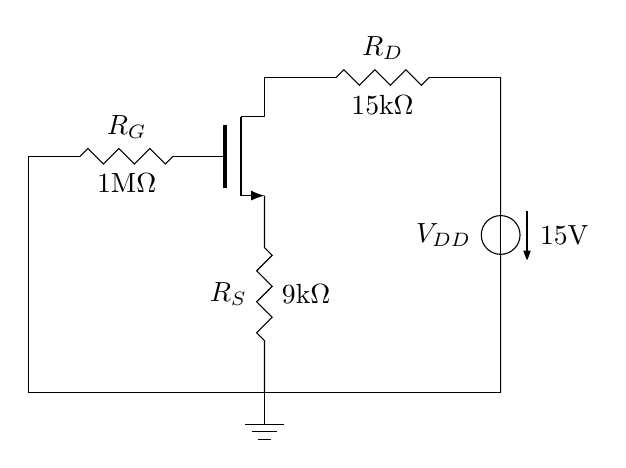
\begin{tikzpicture}[circuit ee IEC,set resistor graphic=var resistor IEC graphic]
\draw (-0.5,0) to [resistor={ohm=1M,info'=$R_G$}] (-3,0);
\draw (-3,0) -- (-3,-3);
\draw (3,1) to [voltage source={direction info={volt=15},info'=$V_{DD}$}] (3,-3);
\draw (3,1) to [resistor={ohm=15k,info'=$R_D$}] (0,1);
\draw (0,-0.5) to [resistor={ohm=9k,info'=$R_S$}] (0,-3);
\draw [very thick] (-0.5,0.4) -- (-0.5,-0.4);
\draw (-3,-3) -- (3,-3) (0,1) -- (0,0.5) -- (-0.3, 0.5);
\draw[-{Latex}] (-0.3,-0.5) -- (0,-0.5);
\draw[thick] (-0.3,0.5) -- (-0.3,-0.5);
\draw (0,-3.5) node (gnd) [ground,point down] {};
\draw (gnd) -- (0,-3);
\end{tikzpicture}
\end{center}

According to the equations,
$$I_D=\frac{K_n}{2}(V_{GS}-V_{TN})^2$$
$$V_{GS}+I_DR_s=0$$

We can get $$V_{GS}+\frac{K_nR_s}{2}(V_{GS}-V_{TN})^2=0$$
$$V_{GS}=V_{TN}=\frac{1}{K_nR_s}\left(\sqrt{1-2K_nR_sV_{TN}}-1\right)$$
\begin{align*}
I_D&=\frac{1}{2K_nR_s^2}\left(\sqrt{1-2K_nR_sV_{TN}}-1\right)^2\\
&=\frac{1}{2\cdot0.3\unit{A/V^2}\cdot(9\unit{k\Omega})^2}\left(\sqrt{1-2\cdot0.3\unit{A/V^2}\cdot9\unit{k\Omega}\cdot-3\unit{V}}-1\right)^2\\
&\approx0.33\unit{mA}
\end{align*}
$$V_{DS}=V_{DD}-I_D(R_D+R_S)=15\unit{V}-0.33\unit{mA}\cdot(15\unit{k\Omega}+9\unit{k\Omega})=7.08\unit{V}$$
\begin{align*}
V_{GS}-V_{TN}&=\frac{1}{K_nR_s}\left(\sqrt{1-2K_nR_sV_{TN}}-1\right)\\
&=\frac{1}{\cdot0.3\unit{A/V^2}\cdot9\unit{k\Omega}}\left(\sqrt{1-2\cdot0.3\unit{A/V^2}\cdot9\unit{k\Omega}\cdot-3\unit{V}}-1\right)\\
&\approx0.047\unit{V}<V_{DS}
\end{align*}

So the $Q$ point is $(0.33\unit{mA},\ 7.08\unit{V})$, and it is in the saturated region.

\item For $Q_1$, the dc equivalent circuit is
\begin{center}
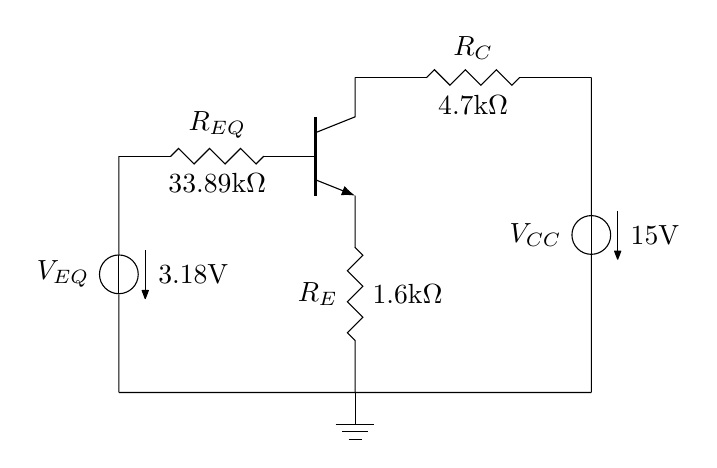
\begin{tikzpicture}[circuit ee IEC,set resistor graphic=var resistor IEC graphic]
\draw (-0.5,0) to [resistor={ohm=33.89k,info'=$R_{EQ}$}] (-3,0);
\draw (-3,0) to [voltage source={direction info={volt=3.18},info'=$V_{EQ}$}] (-3,-3);
\draw (3,1) to [voltage source={direction info={volt=15},info'=$V_{CC}$}] (3,-3);
\draw (3,1) to [resistor={ohm=4.7k,info'=$R_C$}] ( 0,1);
\draw (0,-0.5) to [resistor={ohm=1.6k,info'=$R_E$}] (0,-3);
\draw [very thick] (-0.5,0.5) -- (-0.5,-0.5);
\draw (-3,-3) -- (3,-3) (0,1) -- (0,0.5) -- (-0.5, 0.3);
\draw[-{Latex}] (-0.5,-0.3) -- (0,-0.5);
\draw (0,-3.5) node (gnd) [ground,point down] {};
\draw (gnd) -- (0,-3);
\end{tikzpicture}
\end{center}

Suppose $V_{BE}=0.7V$,
$$I_C=\frac{V_{EQ}-V_{BE}}{\dfrac{R_{EQ}}{\beta_F}+\dfrac{\beta_F+1}{\beta_F}R_E}=\frac{3.18\unit{V}-0.7\unit{V}}{\dfrac{33.89\unit{k\Omega}}{17}+\dfrac{17+1}{17}\cdot1.6\unit{k\Omega}}\approx0.673\unit{mA}$$
$$I_E=\frac{V_{EQ}-V_{BE}}{\dfrac{R_{EQ}}{\beta_F+1}+R_E}=\frac{3.18\unit{V}-0.7\unit{V}}{\dfrac{33.89\unit{k\Omega}}{17+1}+1.6\unit{k\Omega}}\approx0.712\unit{mA}$$
$$V_{CE}=V_{CC}-I_CR_C-I_ER_E=15\unit{V}-0.673\unit{mA}\cdot4.7\unit{k\Omega}-0.712\unit{mA}\cdot1.6\unit{k\Omega}\approx10.70\unit{V}$$

So the $Q$ point is $(0.673\unit{mA},\ 10.70\unit{V})$.

\item For $Q_2$, the dc equivalent circuit is
\begin{center}
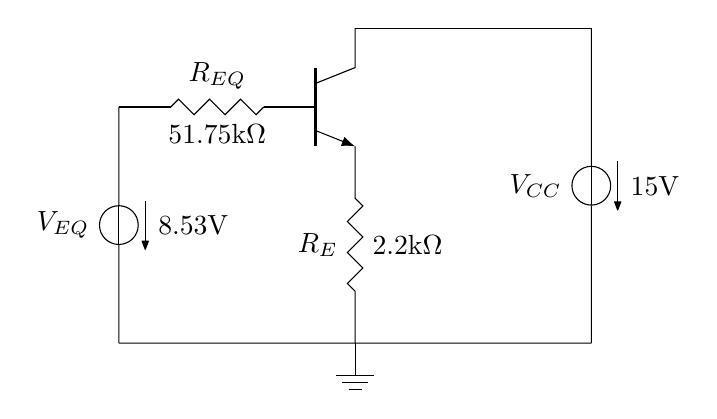
\begin{tikzpicture}[circuit ee IEC,set resistor graphic=var resistor IEC graphic]
\draw (-0.5,0) to [resistor={ohm=51.75k,info'=$R_{EQ}$}] (-3,0);
\draw (-3,0) to [voltage source={direction info={volt=8.53},info'=$V_{EQ}$}] (-3,-3);
\draw (3,1) to [voltage source={direction info={volt=15},info'=$V_{CC}$}] (3,-3);
\draw (3,1) -- (0,1);
\draw (0,-0.5) to [resistor={ohm=2.2k,info'=$R_E$}] (0,-3);
\draw [very thick] (-0.5,0.5) -- (-0.5,-0.5);
\draw (-3,-3) -- (3,-3) (0,1) -- (0,0.5) -- (-0.5, 0.3);
\draw[-{Latex}] (-0.5,-0.3) -- (0,-0.5);
\draw (0,-3.5) node (gnd) [ground,point down] {};
\draw (gnd) -- (0,-3);
\end{tikzpicture}
\end{center}

Suppose $V_{BE}=0.7V$,
$$I_C=\frac{V_{EQ}-V_{BE}}{\dfrac{R_{EQ}}{\beta_F}+\dfrac{\beta_F+1}{\beta_F}R_E}=\frac{8.53\unit{V}-0.7\unit{V}}{\dfrac{51.75\unit{k\Omega}}{23}+\dfrac{23+1}{23}\cdot2.2\unit{k\Omega}}\approx1.723\unit{mA}$$
$$I_E=\frac{V_{EQ}-V_{BE}}{\dfrac{R_{EQ}}{\beta_F+1}+R_E}=\frac{8.53\unit{V}-0.7\unit{V}}{\dfrac{51.75\unit{k\Omega}}{23+1}+2.2\unit{k\Omega}}\approx1.797\unit{mA}$$
$$V_{CE}=V_{CC}-I_CR_C-I_ER_E=15\unit{V}-1.723\unit{mA}\cdot0\unit{k\Omega}-1.797\unit{mA}\cdot2.2\unit{k\Omega}\approx11.05\unit{V}$$

So the $Q$ point is $(1.723\unit{mA},\ 11.05\unit{V})$.

\end{enumerate}

Then we should calculate the small signal parameters.

For $M_1$, $$g_{m1}=\frac{2I_D}{V_{GS}-V_{TN}}=\frac{2\cdot0.33\unit{mA}}{0.047\unit{V}}\approx0.014\unit{S}$$
$$r_{o1}=\frac{1/\lambda+V_{DS}}{I_D}=\frac{1/0.01\times10^{-2}\unit{V^{-1}}+7.08\unit{V}}{0.33\unit{mA}}\approx30.32\unit{M\Omega}$$

For $Q_1$, $$g_{m2}=\frac{I_C}{V_T}=\frac{0.673\unit{mA}}{0.025\unit{V}}\approx0.027\unit{S}$$
$$r_{\pi2}=\frac{\beta_{F1}}{g_{m2}}=\frac{17}{0.027\unit{S}}\approx629\unit{\Omega}$$
$$r_{o2}=\frac{V_{A1}+V_{CE}}{I_C}=\frac{50\unit{V}+10.70\unit{V}}{0.673\unit{mA}}\approx90\unit{k\Omega}$$

For $Q_2$, $$g_{m3}=\frac{I_C}{V_T}=\frac{1.723\unit{mA}}{0.025\unit{V}}\approx0.069\unit{S}$$
$$r_{\pi3}=\frac{\beta_{F2}}{g_{m3}}=\frac{23}{0.069\unit{S}}\approx333\unit{\Omega}$$
$$r_{o3}=\frac{V_{A2}+V_{CE}}{I_C}=\frac{35\unit{V}+11.05\unit{V}}{1.723\unit{mA}}\approx27\unit{k\Omega}$$

The voltage gain:
$$A_{vt1}^{CS}\approx-g_{m1}(R_{D1}\parallel R_{B2}\parallel r_{\pi2})=-0.014\unit{S}\cdot(15\parallel(160\parallel43)\parallel0.629)\unit{k\Omega}\approx-8.30$$
\begin{align*}
A_{vt2}^{CE}&\approx-g_{m2}(R_{C2}\parallel R_{B3}\parallel r_{\pi3}+(1+\beta_{F2})(R_{E3}\parallel R_L))\\
&=-0.027\unit{S}\cdot(4.7\parallel(91\parallel110)\parallel(24\cdot(2.2\parallel0.25)))\unit{k\Omega}\\
&\approx-64.52
\end{align*}
$$A_{vt3}^{CC}\approx\frac{g_{m3}(R_{E3}\parallel R_L)}{1+g_{m3}(R_{E3}\parallel R_L)}=\frac{0.069\unit{S}\cdot(2.2\parallel0.25)\unit{k\Omega}}{1+0.069\unit{S}\cdot(2.2\parallel0.25)\unit{k\Omega}}\approx0.94$$
$$A_v=A_{vt1}^{CS}\cdot A_{vt2}^{CE}\cdot A_{vt3}^{CC}\cdot\frac{R_G}{R_I+R_G}=-8.30\cdot-64.52\cdot0.94\cdot\frac{1\unit{m\Omega}}{10\unit{k\Omega}+1\unit{m\Omega}}\approx498$$

Input signal range:
$$v_i\leqslant\frac{0.2\cdot(V_{GS1}-V_{TN})}{0.990}\approx9.49\unit{mV}$$
$$v_i\leqslant\frac{5\unit{mV}}{|A_{vt1}|\cdot0.990}=\frac{5\unit{mV}}{8.30\cdot0.990}\approx0.61\unit{mV}$$
$$v_i\leqslant\frac{(1+g_{m3}R_{L3})\cdot5\unit{mV}}{A_{vt1}A_{vt2}\cdot0.990}=\frac{(1+0.069\unit{S}\cdot224.5\unit{\Omega})\cdot5\unit{mV}}{8.30\cdot64.52\cdot0.990}\approx0.156\unit{mV}$$

So $$v_i\leqslant0.156\unit{mV}$$

\section{}
First we should apply dc analysis to the circuit, it can be divided into three circuits.

In the first circuit, the dc equivalent circuit is
\begin{center}
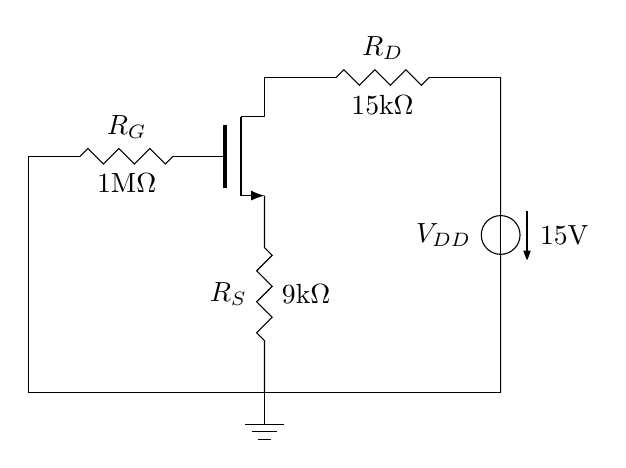
\begin{tikzpicture}[circuit ee IEC,set resistor graphic=var resistor IEC graphic]
\draw (-0.5,0) to [resistor={ohm=1M,info'=$R_G$}] (-3,0);
\draw (-3,0) -- (-3,-3);
\draw (3,1) to [voltage source={direction info={volt=15},info'=$V_{DD}$}] (3,-3);
\draw (3,1) to [resistor={ohm=15k,info'=$R_D$}] (0,1);
\draw (0,-0.5) to [resistor={ohm=9k,info'=$R_S$}] (0,-3);
\draw [very thick] (-0.5,0.4) -- (-0.5,-0.4);
\draw (-3,-3) -- (3,-3) (0,1) -- (0,0.5) -- (-0.3, 0.5);
\draw[-{Latex}] (-0.3,-0.5) -- (0,-0.5);
\draw[thick] (-0.3,0.5) -- (-0.3,-0.5);
\draw (0,-3.5) node (gnd) [ground,point down] {};
\draw (gnd) -- (0,-3);
\end{tikzpicture}
\end{center}

According to the equations,
$$I_D=\frac{K_n}{2}(V_{GS}-V_{TN})^2$$
$$V_{GS}+I_DR_s=0$$

We can get $$V_{GS}+\frac{K_nR_s}{2}(V_{GS}-V_{TN})^2=0$$
$$V_{GS}=V_{TN}=\frac{1}{K_nR_s}\left(\sqrt{1-2K_nR_sV_{TN}}-1\right)$$
\begin{align*}
I_D&=\frac{1}{2K_nR_s^2}\left(\sqrt{1-2K_nR_sV_{TN}}-1\right)^2\\
&=\frac{1}{2\cdot0.9\unit{A/V^2}\cdot(9\unit{k\Omega})^2}\left(\sqrt{1-2\cdot0.9\unit{A/V^2}\cdot9\unit{k\Omega}\cdot-12\unit{V}}-1\right)^2\\
&\approx1.33\unit{mA}
\end{align*}
$$V_{DS}=V_{DD}-I_D(R_D+R_S)=15\unit{V}-1.327\unit{mA}\cdot(15\unit{k\Omega}+9\unit{k\Omega})=-16.92\unit{V}$$
\begin{align*}
V_{GS}-V_{TN}&=\frac{1}{K_nR_s}\left(\sqrt{1-2K_nR_sV_{TN}}-1\right)\\
&=\frac{1}{\cdot0.9\unit{A/V^2}\cdot9\unit{k\Omega}}\left(\sqrt{1-2\cdot0.9\unit{A/V^2}\cdot9\unit{k\Omega}\cdot-12\unit{V}}-1\right)\\
&\approx0.054\unit{V}>V_{DS}
\end{align*}

So it is not in the saturated region, this problem can't be solved.

\section{}

First we should apply dc analysis to the circuit, it can be divided into two circuits.

\begin{enumerate}[(1)]

\item For $Q_1$, the dc equivalent circuit is
\begin{center}
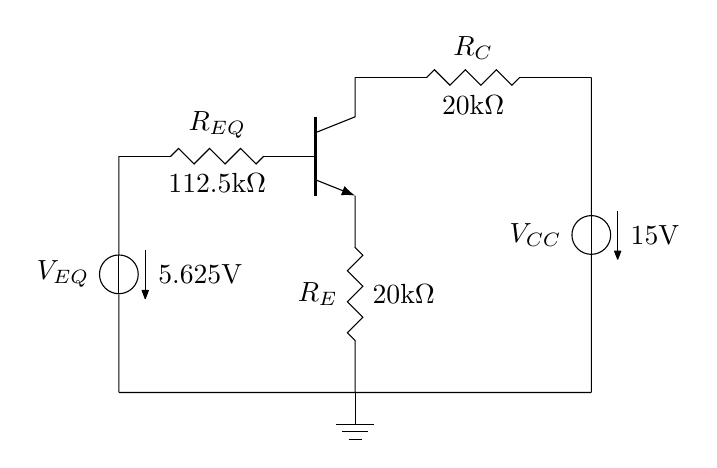
\begin{tikzpicture}[circuit ee IEC,set resistor graphic=var resistor IEC graphic]
\draw (-0.5,0) to [resistor={ohm=112.5k,info'=$R_{EQ}$}] (-3,0);
\draw (-3,0) to [voltage source={direction info={volt=5.625},info'=$V_{EQ}$}] (-3,-3);
\draw (3,1) to [voltage source={direction info={volt=15},info'=$V_{CC}$}] (3,-3);
\draw (3,1) to [resistor={ohm=20k,info'=$R_C$}] ( 0,1);
\draw (0,-0.5) to [resistor={ohm=20k,info'=$R_E$}] (0,-3);
\draw [very thick] (-0.5,0.5) -- (-0.5,-0.5);
\draw (-3,-3) -- (3,-3) (0,1) -- (0,0.5) -- (-0.5, 0.3);
\draw[-{Latex}] (-0.5,-0.3) -- (0,-0.5);
\draw (0,-3.5) node (gnd) [ground,point down] {};
\draw (gnd) -- (0,-3);
\end{tikzpicture}
\end{center}

Suppose $V_{BE}=0.7V$,
$$I_C=\frac{V_{EQ}-V_{BE}}{\dfrac{R_{EQ}}{\beta_F}+\dfrac{\beta_F+1}{\beta_F}R_E}=\frac{5.625\unit{V}-0.7\unit{V}}{\dfrac{112.5\unit{k\Omega}}{300}+\dfrac{300+1}{300}\cdot20\unit{k\Omega}}\approx0.241\unit{mA}$$
$$I_E=\frac{V_{EQ}-V_{BE}}{\dfrac{R_{EQ}}{\beta_F+1}+R_E}=\frac{5.625\unit{V}-0.7\unit{V}}{\dfrac{112.5\unit{k\Omega}}{300+1}+20\unit{k\Omega}}\approx0.242\unit{mA}$$
$$V_{CE}=V_{CC}-I_CR_C-I_ER_E=15\unit{V}-0.241\unit{mA}\cdot20\unit{k\Omega}-0.242\unit{mA}\cdot20\unit{k\Omega}=5.34\unit{V}$$

So the $Q$ point is $(0.241\unit{mA},\ 5.34\unit{V})$.

\item For $Q_2$, the dc equivalent circuit is
\begin{center}
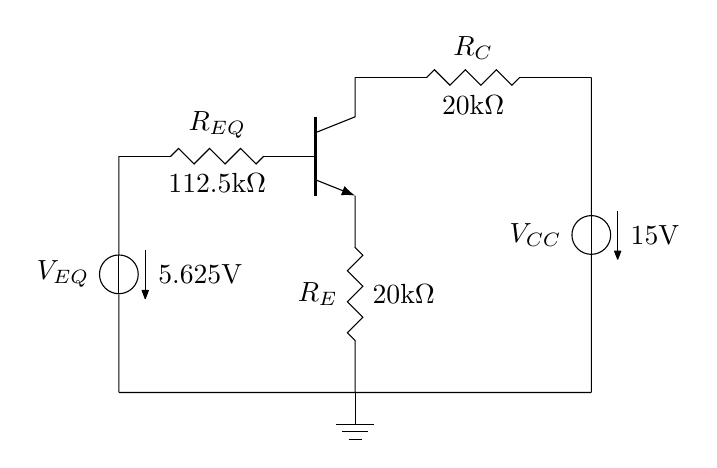
\begin{tikzpicture}[circuit ee IEC,set resistor graphic=var resistor IEC graphic]
\draw (-0.5,0) to [resistor={ohm=112.5k,info'=$R_{EQ}$}] (-3,0);
\draw (-3,0) to [voltage source={direction info={volt=5.625},info'=$V_{EQ}$}] (-3,-3);
\draw (3,1) to [voltage source={direction info={volt=15},info'=$V_{CC}$}] (3,-3);
\draw (3,1) to [resistor={ohm=20k,info'=$R_C$}] ( 0,1);
\draw (0,-0.5) to [resistor={ohm=20k,info'=$R_E$}] (0,-3);
\draw [very thick] (-0.5,0.5) -- (-0.5,-0.5);
\draw (-3,-3) -- (3,-3) (0,1) -- (0,0.5) -- (-0.5, 0.3);
\draw[-{Latex}] (-0.5,-0.3) -- (0,-0.5);
\draw (0,-3.5) node (gnd) [ground,point down] {};
\draw (gnd) -- (0,-3);
\end{tikzpicture}
\end{center}

Suppose $V_{BE}=0.7V$,
$$I_C=\frac{V_{EQ}-V_{BE}}{\dfrac{R_{EQ}}{\beta_F}+\dfrac{\beta_F+1}{\beta_F}R_E}=\frac{5.625\unit{V}-0.7\unit{V}}{\dfrac{112.5\unit{k\Omega}}{42}+\dfrac{42+1}{42}\cdot20\unit{k\Omega}}\approx0.213\unit{mA}$$
$$I_E=\frac{V_{EQ}-V_{BE}}{\dfrac{R_{EQ}}{\beta_F+1}+R_E}=\frac{5.625\unit{V}-0.7\unit{V}}{\dfrac{112.5\unit{k\Omega}}{42+1}+20\unit{k\Omega}}\approx0.217\unit{mA}$$
$$V_{CE}=V_{CC}-I_CR_C-I_ER_E=15\unit{V}-0.213\unit{mA}\cdot20\unit{k\Omega}-0.217\unit{mA}\cdot20\unit{k\Omega}=6.4\unit{V}$$

So the $Q$ point is $(0.213\unit{mA},\ 6.4\unit{V})$.

\end{enumerate}

Then we should calculate the small signal parameters.

For $Q_1$, $$g_{m1}=\frac{I_C}{V_T}=\frac{0.241\unit{mA}}{0.025\unit{V}}=9.64\unit{mS}$$
$$r_{\pi1}=\frac{\beta_{F1}}{g_{m1}}=\frac{300}{9.64\unit{mS}}\approx31.12\unit{k\Omega}$$

For $Q_2$, $$g_{m2}=\frac{I_C}{V_T}=\frac{0.213\unit{mA}}{0.025\unit{V}}=8.52\unit{mS}$$
$$r_{\pi2}=\frac{\beta_{F2}}{g_{m2}}=\frac{42}{8.52\unit{mS}}\approx4.93\unit{k\Omega}$$

Input resistance:
$$R_{in}=r_{\pi1}\parallel R_{B1}=(41.12\parallel180)\unit{k\Omega}\approx33.47\unit{k\Omega}$$

Output resistance:
$$R_{out}=R_L\parallel\left(\frac{1}{g_{m2}}+\frac{R_{C1}\parallel R_{EQ2}}{\beta_{F2}}\right)=100\unit{k\Omega}\parallel\left(\frac{1}{8.52\unit{ms}}+\frac{16.98\unit{k\Omega}}{42}\right)\approx519\unit{\Omega}$$

Midband voltage gain:
$$A_{vt1}^{CE}\approx\frac{-g_{m1}(R_C\parallel R_{EQ}\parallel r_{\pi2})}{1+R_{E1}\cdot g_{m1}}=\frac{-9.64\unit{mS}\cdot(20\parallel112.5\parallel4.93)\unit{k\Omega}}{1+2\unit{k\Omega}\cdot9.64\unit{mS}}=-1.814$$
$$A_{vt2}^{CE}\approx-g_{m2}R_L=-8.52\unit{mS}\cdot(20\parallel100)\unit{k\Omega}=-142$$
$$A_v=A_{vt1}^{CE}\cdot A_{vt2}^{CE}\cdot\frac{R_{in}}{R_I+R_{in}}=-1.814\cdot-142\cdot\frac{33.47\unit{k\Omega}}{(2+33.47)\unit{k\Omega}}\approx243$$
\end{document}

